%%%%
% PLOTS mapas y conglomerados
% bibliografia
%%%%
\usepackage[utf8]{inputenc}
\usepackage{longtable}
\usepackage{authblk}
\usepackage{adjustbox}
\usepackage{natbib}
\title{LOS INDICES DE COLOMBIA}
% autores
\renewcommand\Authand{, y }
\author[1]{\normalsize Emiliano Bojanini}
\affil[1,2]{\small Escuela de Ingenier<U+00ED>a,Universidad de los Andes\\
\texttt{{delcurso,deallado}@uniandes.edu.col}}
\affil[1]{\small Instituto de altas investigaciones financieras\\
Banco del Parque\\
\texttt{delcurso@bp.com.col}}
\date{30 de Junio de 2018}
\usepackage{Sweave}
\begin{document}
\Sconcordance{concordance:ejemplo.tex:ejemplo.Rnw:%
1 19 1 1 0 11 1 1 14 1 4 15 0 1 2 4 1 1 17 1 2 1 1 1 17 1 2 6 1 1 5 12 %
0 1 2 1 6 14 0 1 2 4 1 1 4 1 2 7 1 1 5 1 4 34 0 1 2 6 1 1 9 1 1 1 20 5 %
1 1 19 1 2 7 1}

\maketitle
\begin{abstract}
Este es mi primer trabajo en exploraci<U+00F3>n y modelamiento de indices usando LATEX, R, Anaconda y Zotero.Este es mi primer trabajo en exploraci<U+00F3>n y modelamiento de indices usando LATEX, R, Anaconda y Zotero.Este es mi primer trabajo en exploraci<U+00F3>n y modelamiento de indices usando LATEX, R, Anaconda y Zotero.Este es mi primer trabajo en exploraci<U+00F3>n y modelamiento de indices usando LATEX, R, Anaconda y Zotero.
\end{abstract}
\section*{Introducci<U+00F3>n}
Introducci<U+00F3>n
Aqui les presento mi investigacion sobre diversos estadisticos de Colombia, en el curso de vacaciones de la universidad de los Andes.Aqui les presento mi investigacion sobre diversos estadisticos de Colombia, en el curso de vacaciones de la universidad de los Andes.Aqui les presento mi investigacion sobre diversos estadisticos de Colombia, en el curso de vacaciones de la universidad de los Andes.Aqui les presento mi investigacion sobre diversos estadisticos de Colombia, en el curso de vacaciones de la universidad de los Andes.Aqui les presento mi investigacion sobre diversos estadisticos de Colombia, en el curso de vacaciones de la universidad de los Andes.Aqui les presento mi investigacion sobre diversos estadisticos de Colombia, en el curso de vacaciones de la universidad de los Andes.Aqui les presento mi investigacion sobre diversos estadisticos de Colombia, en el curso de vacaciones de la universidad de los Andes.
\clearpage
\section{Exploraci<U+00F3>n Univariada}\label{univariada}
En esta secci<U+00F3>n exploro cada <U+00ED>ndice.
Para conocer el comportamiento de las variables se ha preparado la Tabla \ref{stats}, donde se estadisticos de cada variable. Los n<U+00FA>meros representan la situaci<U+00F3>n de algun regi<U+00F3>n en ese indicador.
% Table created by stargazer v.5.2.2 by Marek Hlavac, Harvard University. E-mail: hlavac at fas.harvard.edu
% Date and time: Wed, Jul 04, 2018 - 21:50:04
\begin{table}[!htbp] \centering 
  \caption{Medidas estad<U+00ED>sticas} 
  \label{stats} 
\begin{tabular}{@{\extracolsep{5pt}}lccccc} 
\\[-1.8ex]\hline 
\hline \\[-1.8ex] 
Statistic & \multicolumn{1}{c}{N} & \multicolumn{1}{c}{Mean} & \multicolumn{1}{c}{Median} & \multicolumn{1}{c}{Min} & \multicolumn{1}{c}{Max} \\ 
\hline \\[-1.8ex] 
IDH & 32 & 0.802 & 0.804 & 0.691 & 0.879 \\ 
Poblaci..n.Cabecera & 32 & 1,196,730.000 & 717,197 & 13,090 & 10,070,801 \\ 
Poblaci..n.Resto & 32 & 360,590.300 & 268,111.5 & 21,926 & 1,428,858 \\ 
Poblaci..n.Total & 32 & 1,557,320.000 & 1,028,429 & 43,446 & 10,985,285 \\ 
\hline \\[-1.8ex] 
\end{tabular} 
\end{table} % Como apreciamos en la Tabla \ref{Tfrecuencias}, los pa<U+00C3>?ses en la mejor situaci<U+00C3><U+00B3>n son los menos, salvo en el caso del \emph{<U+00C3>?ndice de libertas mundial}\footnote{N<U+00C3><U+00B3>tese que esto se puede deber a la {\bf menor} cantidad de categor<U+00C3>?as.}
Para resaltar lo anterior, tenemos la Figura \ref{barplots} en la p<U+00E1>gina \pageref{barplots}.
%%%%% figure
\begin{figure}[h]
\centering
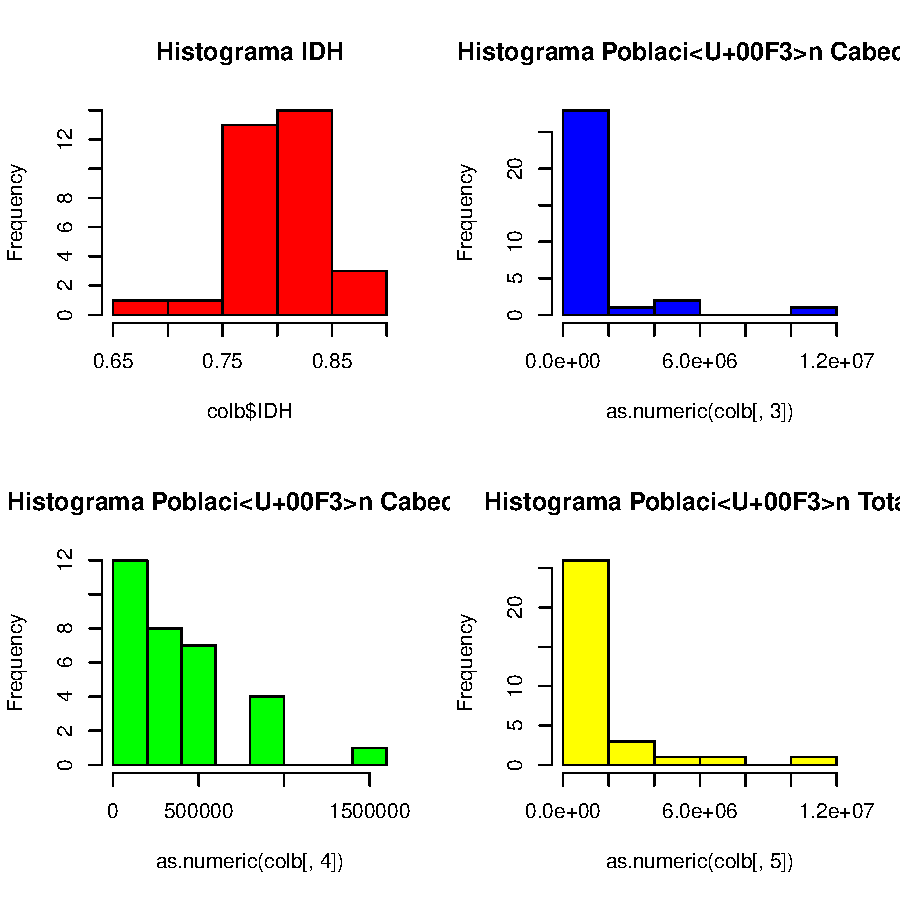
\includegraphics{ejemplo-barplots}
Dado el sesgo de las pobaciones,podriamos transformarla para que se acerque a la normalidad.
\begin{adjustbox}{width=9cm,height=3cm,clip,trim=1.5cm 0.5cm 0cm 1.5cm}
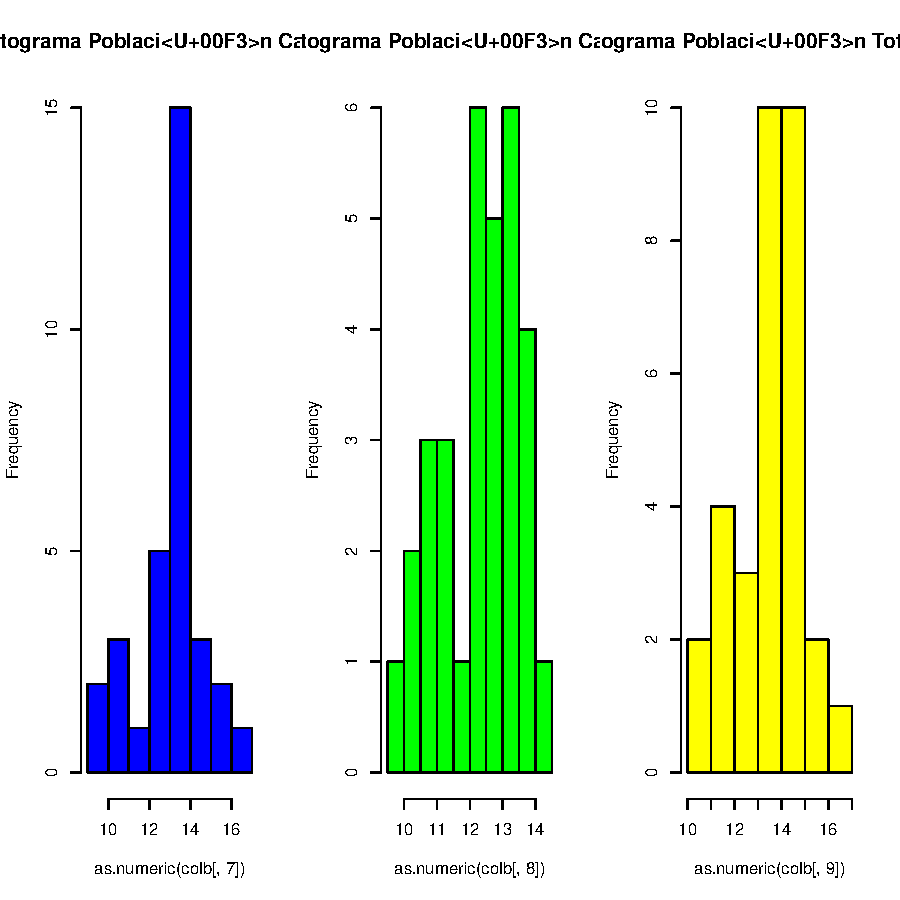
\includegraphics{ejemplo-barplots2}
\end{adjustbox}
\caption{Distribuci<U+00F3>n de Indicadores}
\label{barplots}
\end{figure}
\clearpage
\section{Exploraci<U+00F3>n Bivariada}
En este trabajo estamos interesados en el impacto de la poblacion en el el IDH, veamos IDH con cada uno:
% Table created by stargazer v.5.2.2 by Marek Hlavac, Harvard University. E-mail: hlavac at fas.harvard.edu
% Date and time: Wed, Jul 04, 2018 - 21:50:04
\begin{table}[!htbp] \centering 
  \caption{Correlaci<U+00F3>n de Democracia con las dem<U+00E1>s variables} 
  \label{corrDem} 
\begin{tabular}{@{\extracolsep{5pt}} ccc} 
\\[-1.8ex]\hline 
\hline \\[-1.8ex] 
cabeLog & restoLog & totaLog \\ 
\hline \\[-1.8ex] 
$0.487$ & $0.177$ & $0.424$ \\ 
\hline \\[-1.8ex] 
\end{tabular} 
\end{table} La correlaci<U+00F3>n entre las variables independientes:
% Table created by stargazer v.5.2.2 by Marek Hlavac, Harvard University. E-mail: hlavac at fas.harvard.edu
% Date and time: Wed, Jul 04, 2018 - 21:50:04
\begin{table}[!htbp] \centering 
  \caption{Correlaci<U+00F3>n de Democracia con las dem<U+00E1>s variables} 
  \label{corrTablex} 
\begin{tabular}{@{\extracolsep{5pt}} cccc} 
\\[-1.8ex]\hline 
\hline \\[-1.8ex] 
 & cabeLog & restoLog & totaLog \\ 
\hline \\[-1.8ex] 
cabeLog & 1 &  &  \\ 
restoLog & 0.84 & 1 &  \\ 
totaLog & 0.99 & 0.9 & 1 \\ 
\hline \\[-1.8ex] 
\end{tabular} 
\end{table} Visualmente:
Lo visto en la Tabla \ref{corrTableX} se refuerza claramente en la Figura \ref{corrPlotX}.
\begin{figure}[h]
\centering
\begin{adjustbox}{width=7cm,height=7cm,clip,trim=1.5cm 0.5cm 0cm 1.5cm}
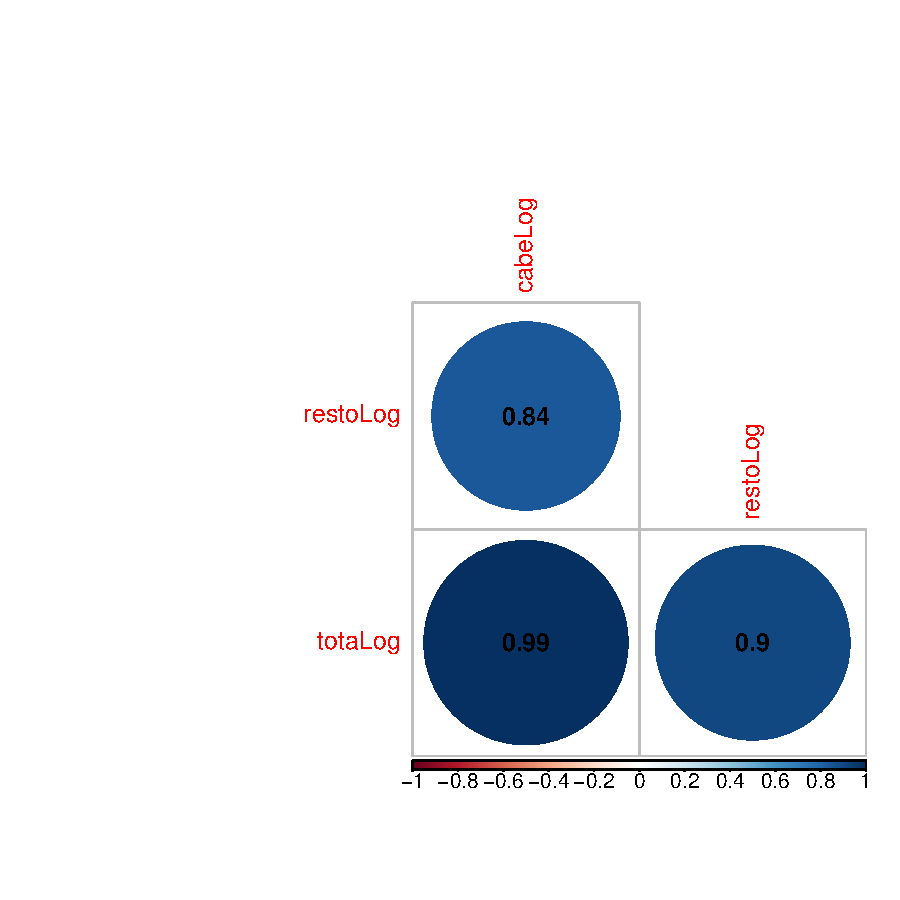
\includegraphics{ejemplo-corrPlotX}
\end{adjustbox}
\caption{correlaci<U+00C3><U+00B3>n entre predictores}
\label{corrPlotX}
\end{figure}
\clearpage
\section{Modelos de Regresi<U+00F3>n}
Veamos los modelos propuestos.
Primero sin poblacion resto, luego con esa:
Resultados
% Table created by stargazer v.5.2.2 by Marek Hlavac, Harvard University. E-mail: hlavac at fas.harvard.edu
% Date and time: Wed, Jul 04, 2018 - 21:50:04
\begin{table}[!htbp] \centering 
  \caption{Modelos de Regresi<U+00F3>n} 
  \label{regresiones} 
\begin{tabular}{@{\extracolsep{5pt}}lcc} 
\\[-1.8ex]\hline 
\hline \\[-1.8ex] 
 & \multicolumn{2}{c}{\textit{Dependent variable:}} \\ 
\cline{2-3} 
\\[-1.8ex] & \multicolumn{2}{c}{IDH} \\ 
\\[-1.8ex] & (1) & (2)\\ 
\hline \\[-1.8ex] 
 cabeLog & 0.013$^{***}$ & 0.066 \\ 
  & (0.004) & (0.046) \\ 
  & & \\ 
 restoLog &  & $-$0.016 \\ 
  &  & (0.020) \\ 
  & & \\ 
 totaLog &  & $-$0.051 \\ 
  &  & (0.064) \\ 
  & & \\ 
 Constant & 0.634$^{***}$ & 0.818$^{***}$ \\ 
  & (0.055) & (0.092) \\ 
  & & \\ 
\hline \\[-1.8ex] 
Observations & 32 & 32 \\ 
R$^{2}$ & 0.238 & 0.437 \\ 
Adjusted R$^{2}$ & 0.212 & 0.377 \\ 
Residual Std. Error & 0.037 (df = 30) & 0.033 (df = 28) \\ 
F Statistic & 9.347$^{***}$ (df = 1; 30) & 7.257$^{***}$ (df = 3; 28) \\ 
\hline 
\hline \\[-1.8ex] 
\textit{Note:}  & \multicolumn{2}{r}{$^{*}$p$<$0.1; $^{**}$p$<$0.05; $^{***}$p$<$0.01} \\ 
\end{tabular} 
\end{table} \clearpage
\section{Exploraci<U+00F3>n Espacial}
Calculemos conglomerados de regiones,usando toda la informaci<U+00F3>n de las tres variables.
Usaremos la tecnica de k-means propuesta por MacQueen.\cite{reynolds_clustering_2006}
Como acabamos de ver en la Tabla \ref{regresiones} en la p<U+00C3><U+00A1>gina \pageref{regresiones}, si quisieras sintetizar la multidimensionalidad de nuestros indicadores, podr<U+00C3>?amos usar tres de las cuatro variables que tenemos (un par de las originales tiene demasiada correlaci<U+00F3>n).
%As<U+00C3>?, propongo que calculemos conglomerados de pa<U+00C3>?ses usando toda la informaci<U+00C3><U+00B3>n de tres de los indicadores. Como nuestras variables son ordinales utilizaremos un proceso de conglomeraci<U+00C3><U+00B3>n donde las distancia ser<U+00C3><U+00A1>n calculadas usando la medida {\bf gower} propuestas en \cite{gower_general_1971}, y para los enlazamientos usaremos la t<U+00C3><U+00A9>cnica de {\bf medoides} seg<U+00C3><U+00BA>n \cite{reynolds_clustering_2006}. Los tres conglomerados se muestran en la Figura \ref{clustmap}.
%
%
%
%
%
%
\begin{figure}[h]
\centering
%\begin{adjustbox}{width=11cm,height=8cm,clip,trim=1cm 2.5cm 0cm 2.5cm}
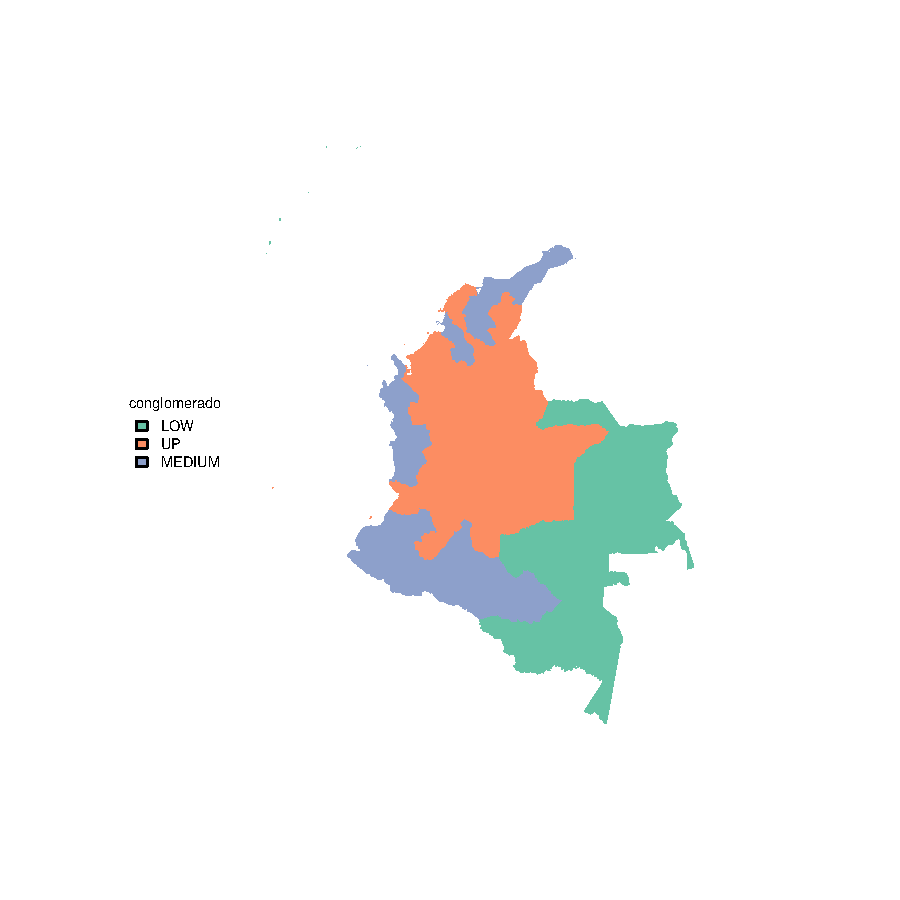
\includegraphics{ejemplo-plotMap1}
%\end{adjustbox}
\caption{Paises conglomerados segun sus indicadores sociopol<U+00C3>?ticos}\label{clustmap}
\end{figure}
%
\bibliographystyle{abbrv}
\renewcommand{\refname}{Bibliography}
\bibliography{Colombia}
\end{document}
